\documentclass{beamer}
\usepackage{graphicx}
\usepackage[inkscapelatex=false]{svg}
\usepackage{tabularx}
\usepackage{siunitx}
\usepackage{booktabs}
\usepackage[normalem]{ulem}
\usepackage{pifont}
\usepackage[export]{adjustbox}
\usepackage{subcaption}
\graphicspath{ {./graphics/}{./Pictures/} }
\usetheme{Madrid}
\definecolor{lightblue}{RGB}{0,73,114}
\definecolor{grund}{RGB}{238,241,251}          
\definecolor{schrift}{RGB}{0,73,114}
\definecolor{magenta}{RGB}{128,0,128}
\definecolor{maroon}{RGB}{113, 41, 21  }
\setbeamercolor{structure}{fg=maroon}

\newcommand*{\thead}[1]{\multicolumn{1}{c}{#1}}
\newcommand{\cmark}{\ding{51}}
\newcommand{\xmark}{\ding{55}}

\title{Blood Pressure Estimation through Photoplethysmography using Deep Learning in Clinical Setting: Critical Survey and Solutions}
\author{François LaBerge}
\institute[]{Concordia University}
\date{April 2024}

\begin{document}

\AtBeginSection[]
{
    \begin{frame}
        \frametitle{Table of Contents}
        \tableofcontents[currentsection]
    \end{frame}
}

\frame{\titlepage}

% IMPACK CPR
% It's an ML regerssion task
% explain random vs patient-wise split
% Training settings+

\section{Introduction}
\begin{frame}{Blood Pressure Monitoring}
    \begin{columns}
        \column{0.5\columnwidth}
        \begin{itemize}

            \item Blood pressure
                  \begin{itemize}
                      \item Pressure against arterial wall
                      \item Systolic and diastolic pressures
                      \item mmHg
                  \end{itemize}


            \item Monitoring
                  \begin{itemize}
                      \item Intraoperative care
                      \item Hypotension \& Hypertension
                  \end{itemize}
        \end{itemize}

        \column{0.5\columnwidth}
        \begin{figure}
            \centering
            
\includegraphics[width=0.5\columnwidth]{introduction/bp.jpg}
            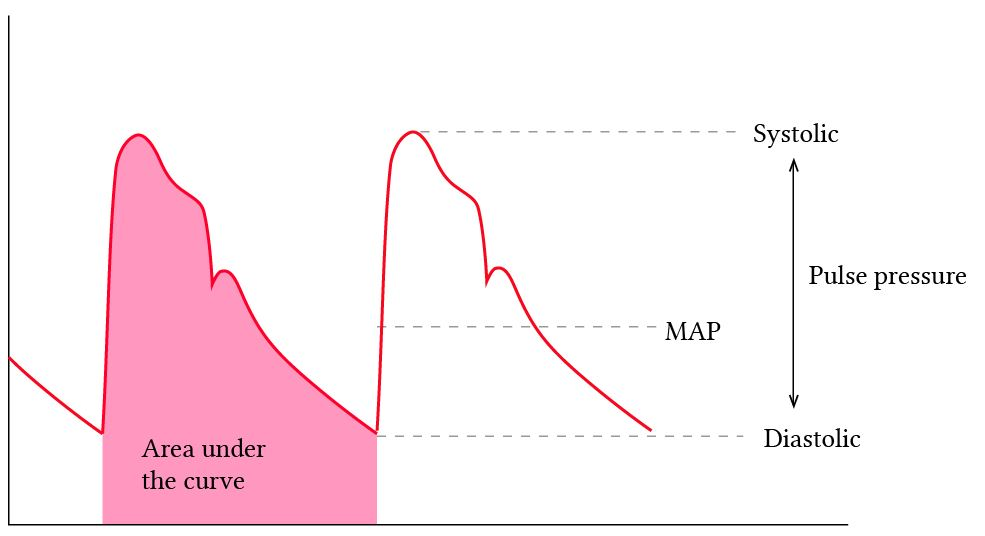
\includegraphics[width=\columnwidth]{introduction/systolicdiastolic.png}
        \end{figure}
    \end{columns}


\end{frame}

\begin{frame}{Context}{Application}
    \begin{columns}
        \column{0.5\columnwidth}
        \centering
        Clinical
        \begin{figure}
            \centering
            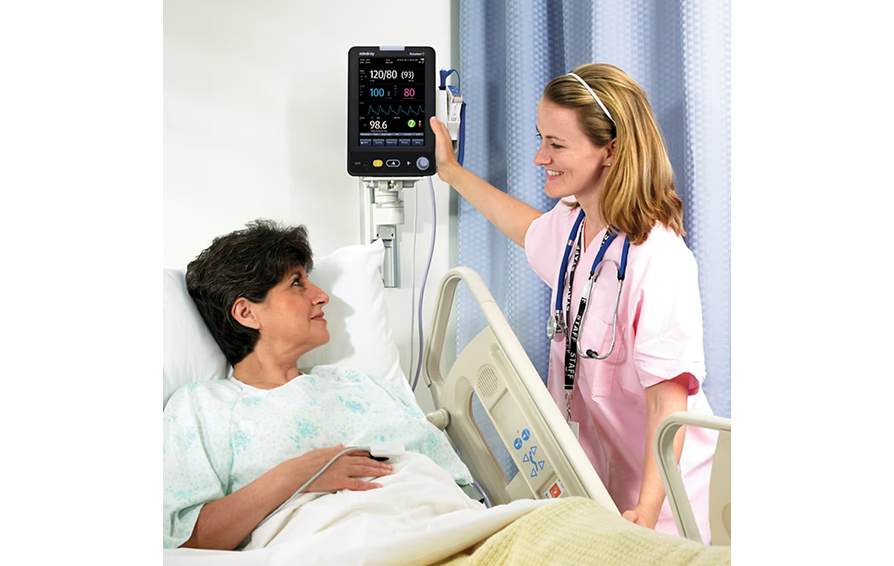
\includegraphics[width=\columnwidth]{introduction/clinical.png}
        \end{figure}

        \column{0.5\columnwidth}
        \centering
        EMS
        \begin{figure}
            \centering
            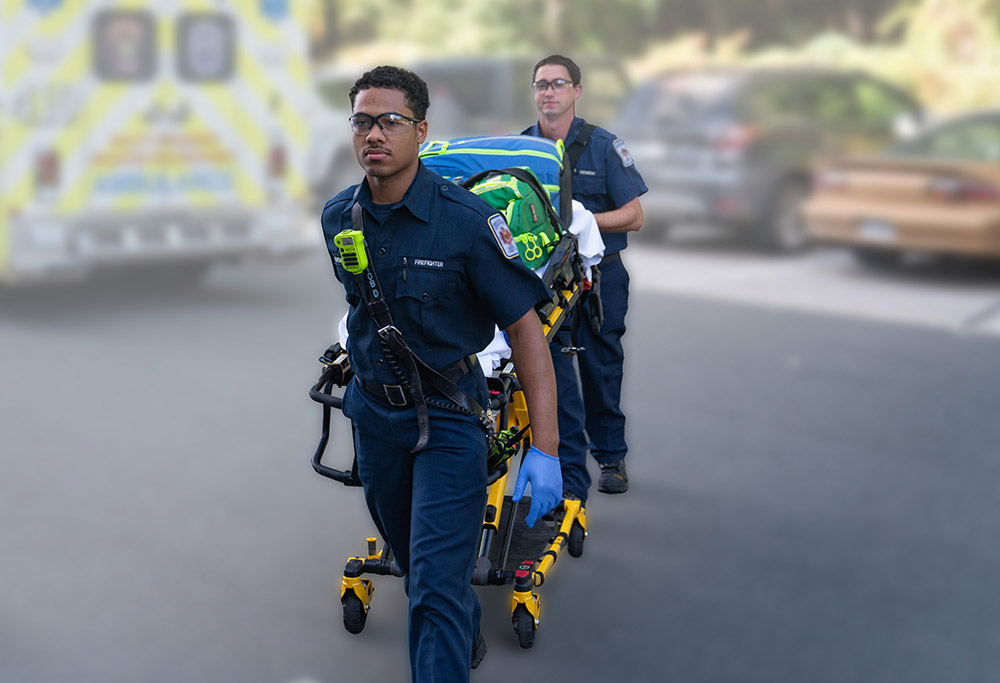
\includegraphics[width=\columnwidth]{introduction/ems.jpg}
        \end{figure}
    \end{columns}
\end{frame}

\begin{frame}{Context}{Sponsor}
    \begin{columns}
        \column{0.5\columnwidth}
        \begin{itemize}
            \item IMPACK CPR
            \item Chest Compression Device
            \item Feedback loop with vital signs
        \end{itemize}
        \begin{figure}
            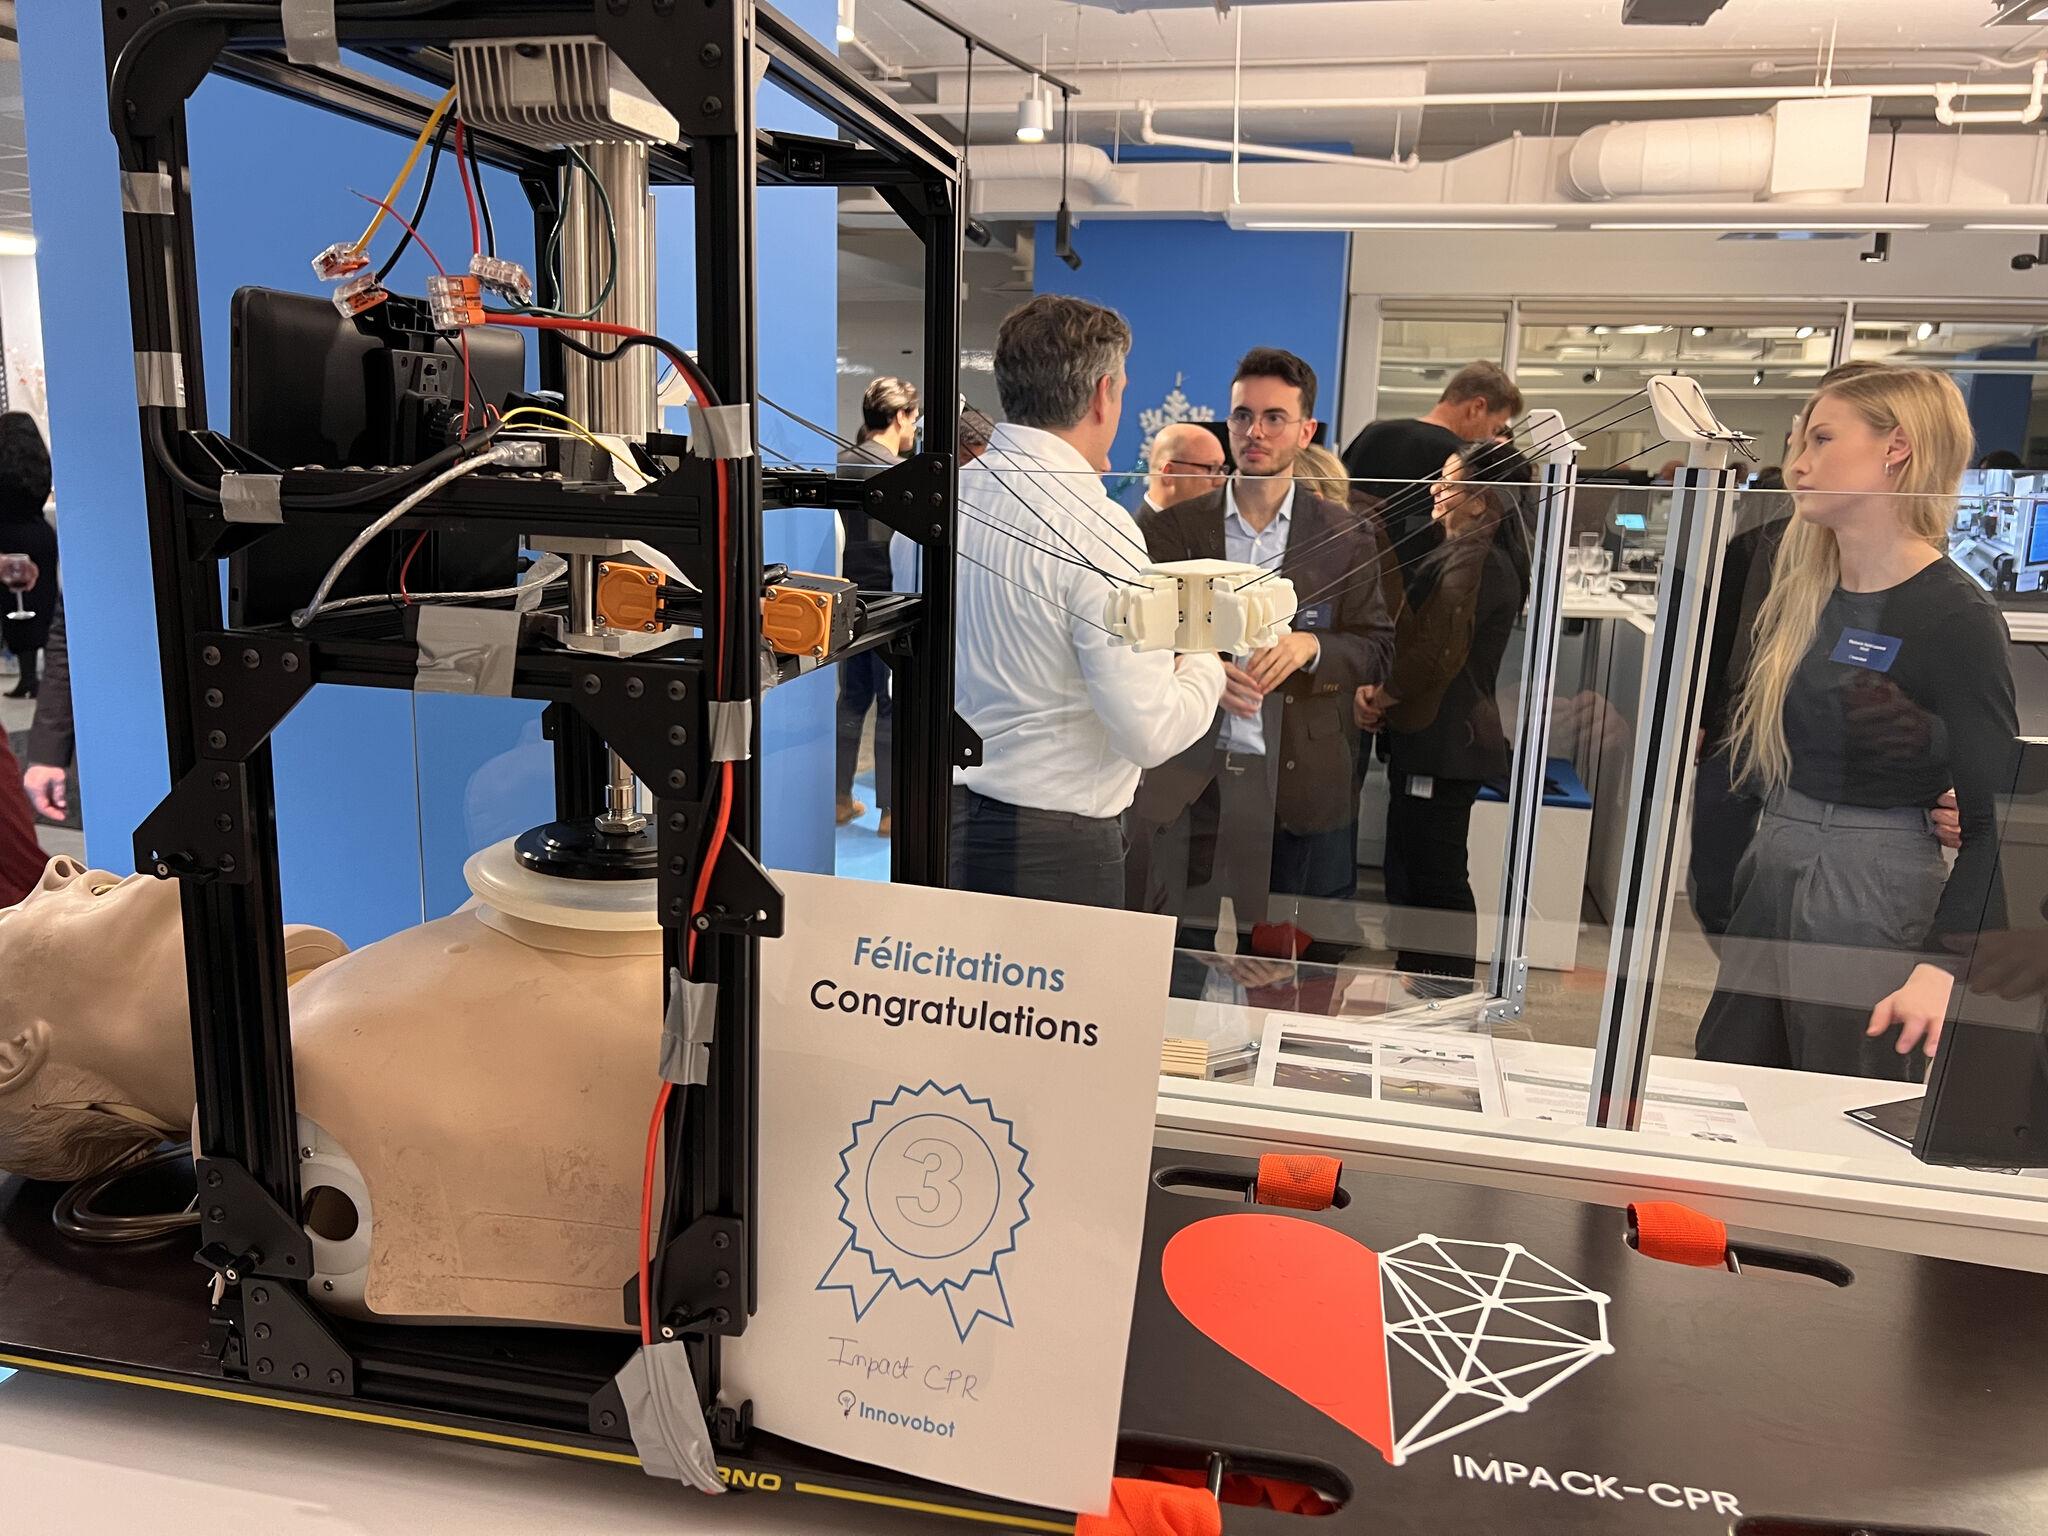
\includegraphics[width=\columnwidth]{introduction/massseur.jpeg}
        \end{figure}

        \column{0.5\columnwidth}
        \begin{figure}
            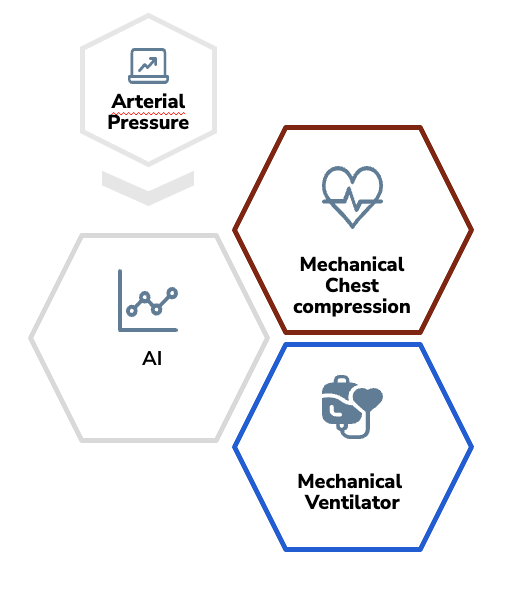
\includegraphics[width=\columnwidth]{introduction/loop.png}
        \end{figure}

    \end{columns}

\end{frame}

\begin{frame}{Current Solutions}
    \begin{columns}
        \column{0.5\columnwidth}
        \centering
        Cuff-based
        \begin{figure}
            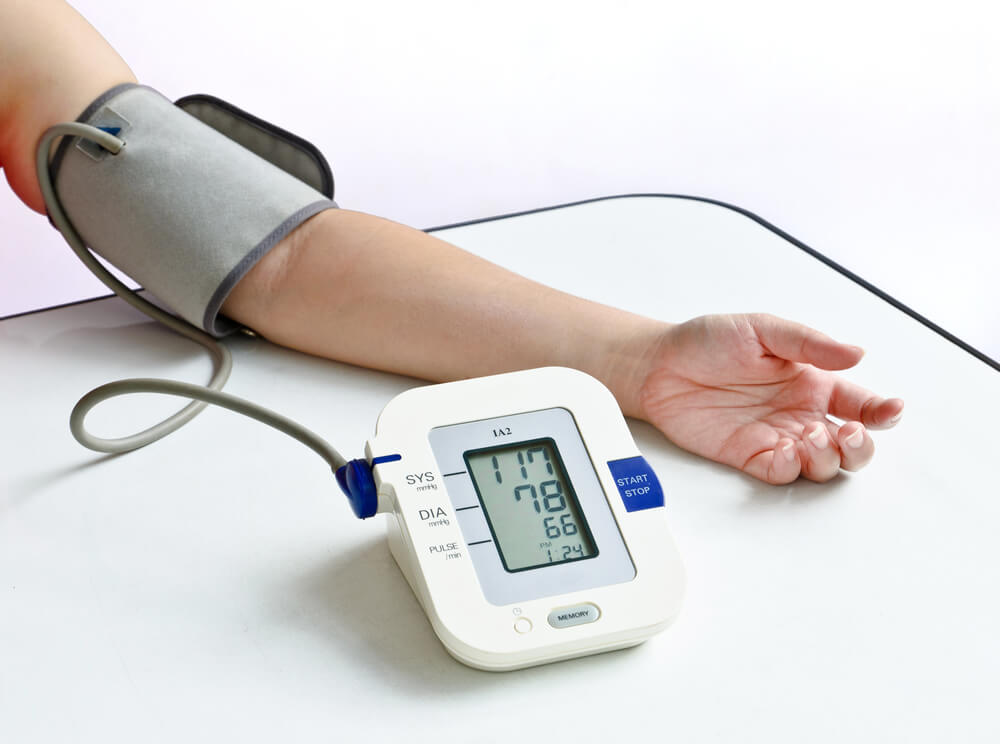
\includegraphics[width=\columnwidth]{introduction/cuff.jpg}
        \end{figure}
        % \begin{itemize}
        %     \item + non-invasive
        %     \item - not continuous
        % \end{itemize}

        \column{0.5\columnwidth}
        \centering
        Catheterization
        \begin{figure}
            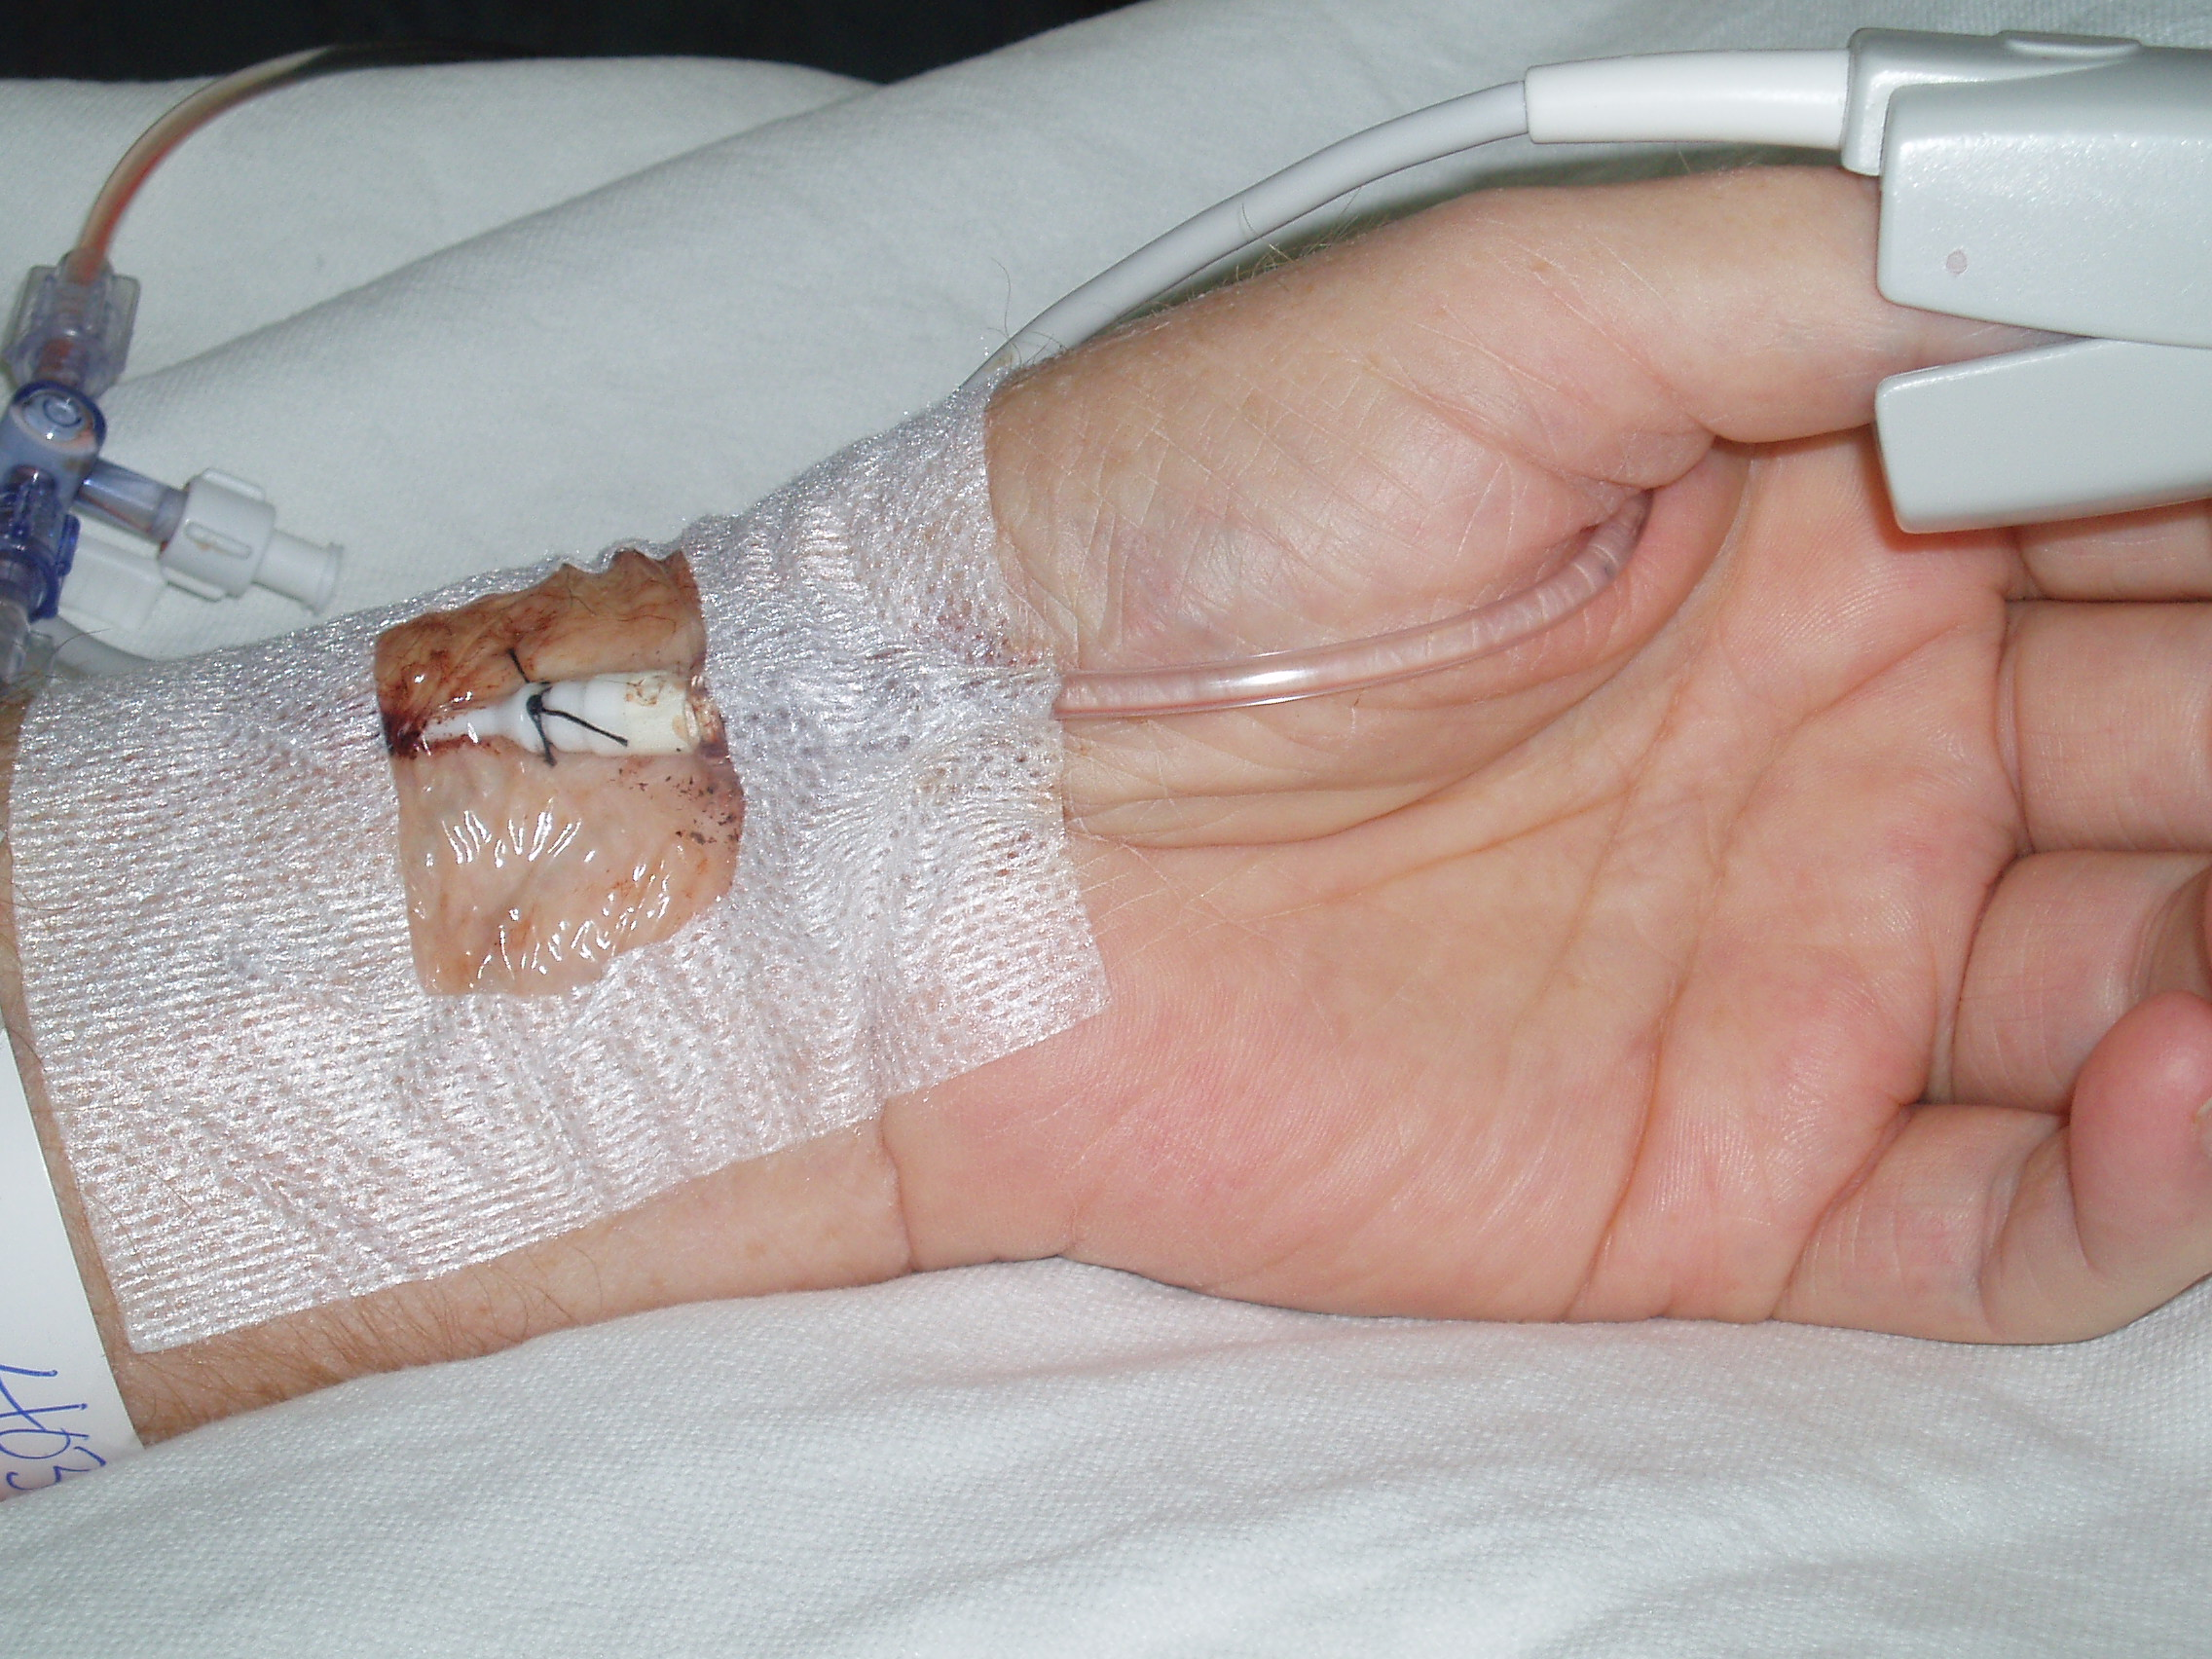
\includegraphics[width=\columnwidth]{introduction/catheter.jpeg}
        \end{figure}
        % \begin{itemize}
        %     \item - invasive
        %     \item + continuous
        % \end{itemize}
    \end{columns}
    \begin{table}
        \begin{tabular}{r c c}
            \hline
                       & non-invasive & continuous \\
            \hline
            cuff-based & \cmark       & \xmark     \\
            catheter   & \xmark       & \cmark     \\
            \hline
        \end{tabular}
    \end{table}
\end{frame}

\begin{frame}{Goal}
    Properties of the desired system
    \begin{table}
        \begin{tabular}{r c c}
            \hline
                           & non-invasive & continuous \\
            \hline
            cuff-based     & \cmark       & \xmark     \\
            catheter       & \xmark       & \cmark     \\
            desired system & \cmark       & \cmark     \\
            \hline
        \end{tabular}
    \end{table}
    Improve outcomes for patients
\end{frame}

\section{Literature Review}
\begin{frame}{Photoplethysmography (PPG)}
    \begin{columns}
        \column{0.5\columnwidth}
        \begin{itemize}
            \item Light-based method
            \item Measures the volume of blood
            \item Similar signal to ABP
        \end{itemize}

        \column{0.5\columnwidth}
        \begin{figure}
            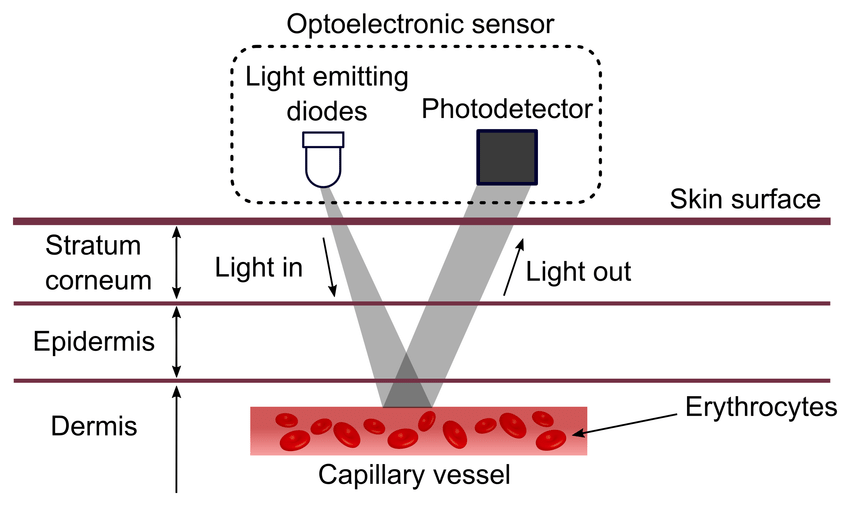
\includegraphics[width=0.6\columnwidth]{literature/ppgdiagram.png}
            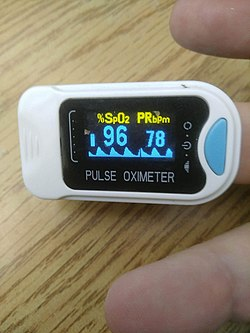
\includegraphics[width=0.3\columnwidth]{literature/ppgfinger.png}
        \end{figure}
    \end{columns}
    \begin{figure}
        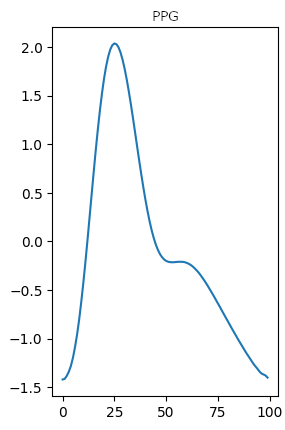
\includegraphics[width=0.25\columnwidth]{literature/signalppg.png}
        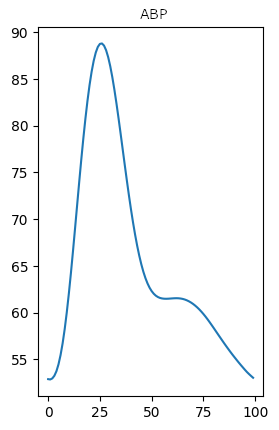
\includegraphics[width=0.25\columnwidth]{literature/singalabp.png}
    \end{figure}

\end{frame}

\begin{frame}{ML \& DL approaches}
    \begin{itemize}
        \item PPG $\to$ ABP
        \item Regression task
        \item Association for the Advancement of Medical Instrumentation (AAMI): $5\pm8$ mmHg ($MAE \pm SD$)
    \end{itemize}
    \begin{figure}
        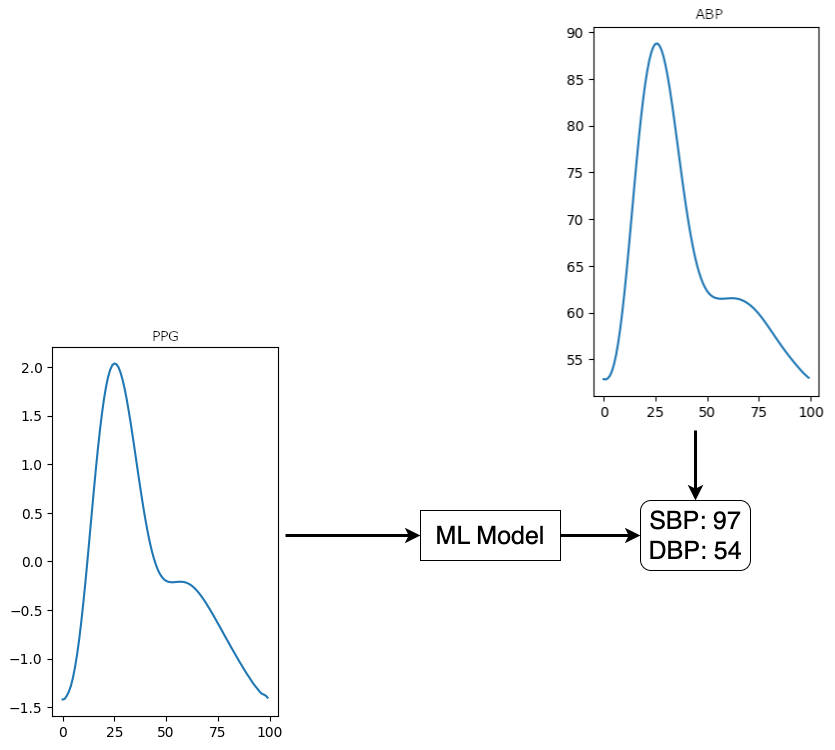
\includegraphics[width=0.5\columnwidth]{literature/regression.png}
    \end{figure}
\end{frame}

\begin{frame}{Dataset split}
    \begin{itemize}
        \item Dataset split is ambiguous
        \item Random split $\to$ data leakage
        \item Learn the physiology of a patient
        \item Patient-wise split is required
        \item Personalization is not applicable
    \end{itemize}
    \begin{figure}
        \centering
        Random split \medskip \par
        \includesvg[width=0.7\columnwidth]{literature/randomsplit.svg}

        \medskip

        Patient-wise split \medskip \par
        \includesvg[width=0.7\columnwidth]{literature/patientwisesplit.svg}
    \end{figure}
\end{frame}

\begin{frame}{Calibration-free}
    New property of the desired solution
    \begin{table}
        \begin{tabular}{r c c c}
            \hline
                             & non-invasive & continuous & calibration-free \\
            \hline
            cuff-based       & \cmark       & \xmark     & \cmark           \\
            catheter         & \xmark       & \cmark     & \cmark           \\
            ML w/ pers.      & \cmark       & \cmark     & \xmark           \\
            desired solution & \cmark       & \cmark     & \cmark           \\
            \hline
        \end{tabular}
    \end{table}
\end{frame}

\begin{frame}{Literature Gaps}
    Difficulty in comparing articles
    \begin{itemize}
        \item Dataset is not shared
        \item Preprocessing can not be reproduced
        \item Model implementations are not published
        \item Inconsistent performance metrics
    \end{itemize}
\end{frame}

\section{Contributions}

\subsection{Survey}
\begin{frame}{Contribution 1: Survey}
    \begin{block}{Objective}
        We first provide a comprehensive review of the literature through a survey.
    \end{block}
\end{frame}

\begin{frame}{Contribution 1: Survey}{Methodology}
    \begin{columns}
        \column{0.5\textwidth}
        Search Engines (3)
        \begin{itemize}
            \item Google Scholar
            \item PubMed's search engine
            \item Sofia
            \item IEEE
            \item SCOPUS
        \end{itemize}

        \column{0.5\textwidth}
        Keywords (19)
        \begin{itemize}
            \item machine learning
            \item deep learning
            \item ABP
            \item estimation
            \item PPG
            \item continuous
            \item non-invasive
            \item cuffless
            \item etc.
        \end{itemize}
    \end{columns}

    \pause
    \vspace{1cm}
    \centering
    \alert{50 articles, 176 models}
\end{frame}

\begin{frame}{Contribution 1: Survey}{Methodology}
    \begin{itemize}
        \item Annotate articles
              \begin{itemize}
                  \item Dataset
                  \item Preprocessing
                  \item Model architecture
                  \item Performance
                  \item etc.
              \end{itemize}
        \item Extract statistics
    \end{itemize}
    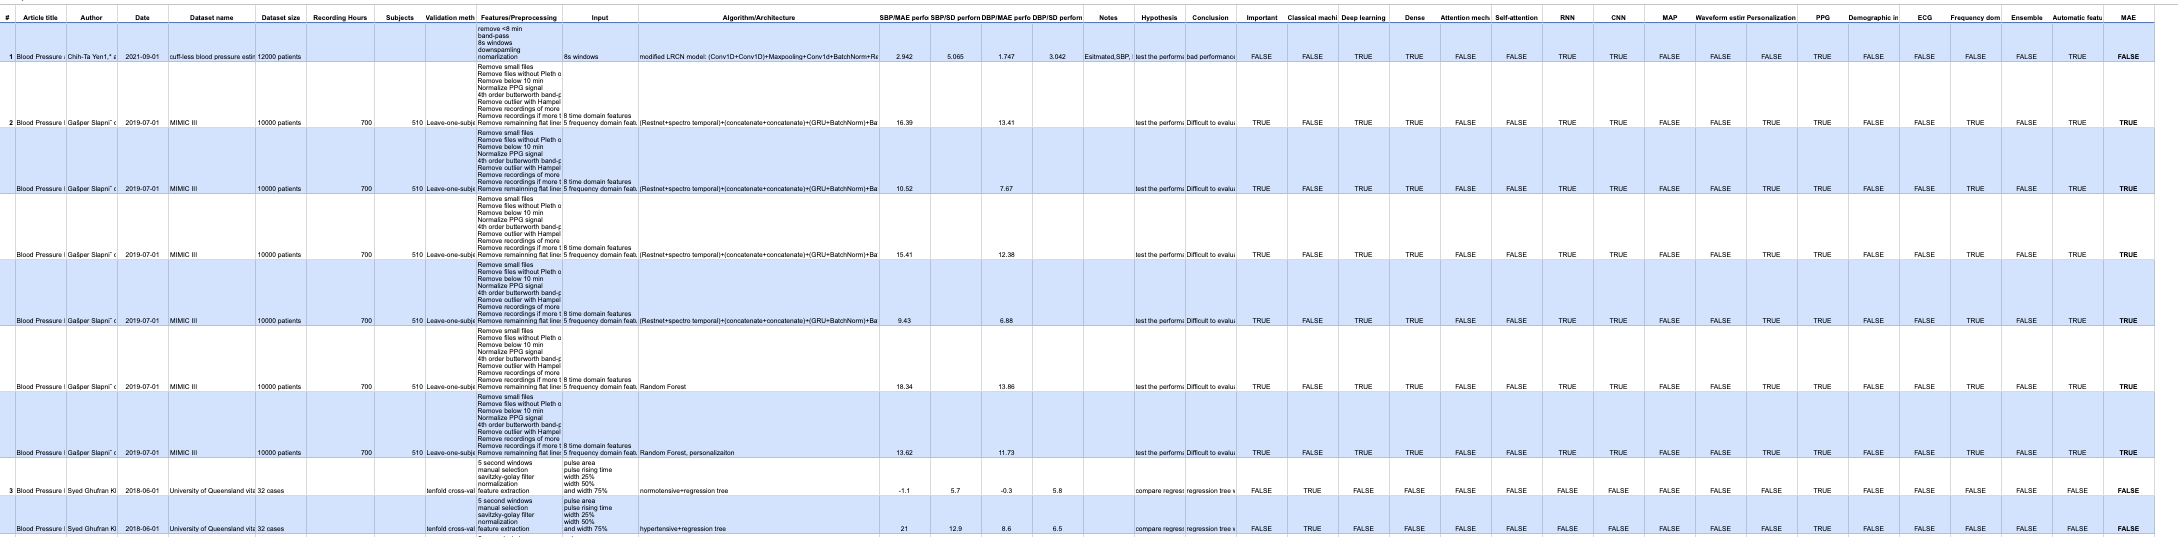
\includegraphics[width=\textwidth]{survey/bigtable.png}
    \href{https://docs.google.com/spreadsheets/u/1/d/e/2PACX-1vR-3MoAcaD-N30ZM15ozSlxh8RHTUBv2KETb9f2g852htlH-5PNt_S8khVnUFLWeEo2H91ZW9hCEi8o/pubhtml}{published online for viewing}
\end{frame}

\begin{frame}{Contribution 1: Survey}{Results}
    Taxonomy of approaches
    \begin{figure}
        \includesvg[scale=0.6]{survey/Taxonomy.drawio.svg}
    \end{figure}
\end{frame}

\begin{frame}{Contribution 1: Survey}{Results}
    Methods
    \begin{figure}
        \includesvg[width=0.3\columnwidth]{survey/input.svg}
        \hfill
        \includesvg[width=0.3\columnwidth]{survey/algorithm.svg}
        \hfill
        \includesvg[width=0.3\columnwidth]{survey/layers.svg}
    \end{figure}
    \begin{itemize}
        \item PPG
        \item Deep Learning
        \item Dense, RNN, CNN
    \end{itemize}
\end{frame}

\begin{frame}{Contribution 1: Survey}{Results}
    Years
    \begin{columns}
        \column{0.7\columnwidth}
        \begin{figure}
            \includesvg[width=\columnwidth]{survey/years.svg}
        \end{figure}

        \column{0.3\columnwidth}
        \begin{itemize}
            \item Almost all after 2018
        \end{itemize}
    \end{columns}


\end{frame}

\begin{frame}{Contribution 1: Survey}{Results}
    Reported Performance

    \begin{figure}
        \includesvg[width=0.49\columnwidth]{survey/mae.svg}
        \includesvg[width=0.49\columnwidth]{survey/sd.svg}
    \end{figure}

    \begin{itemize}
        \item 36 SBP
        \item 54 DBP
        \item 36 SBP \& DBP, $32\%$
    \end{itemize}
\end{frame}

\begin{frame}{Contribution 1: Survey}{Results}
    % TODO move right
    Filter articles based on annotations
    \begin{itemize}
        \item PPG Only
        \item Automatic Feature Extraction
        \item Public datasets only
        \item MAE performance metric
    \end{itemize}

    \pause
    \alert{8 articles, 9 models}
\end{frame}

\begin{frame}{Contribution 1: Survey}{Results}
    \begin{table}
        \centering
        \tiny
        \begin{tabularx}{\textwidth}{ l >{\raggedright\arraybackslash}X l >{\raggedright\arraybackslash}X }
            \hline
            No. & \thead{Authors}                                 & \thead{Architecture}                                             \\
            \hline
            1   & Slapničar et al. \cite{slapnicar_blood_2019}    & spectro-temporal ResNet inspired                                 \\
            2   & Athaya and Choi \cite{athaya_estimation_2021}   & U-Net inspired                                                   \\
            3   & Chen et al. \cite{chen_new_2022}                & RSPAN                                                            \\
            4   & Harfiya et al. \cite{harfiya_continuous_2021}   & LSTM autoencoder                                                 \\
            5   & Kim et al. \cite{kim_deepcnap_2022}             & ResUNet with attention-based skip connections and self-attention \\
            6   & Leitner et al. \cite{leitner_personalized_2022} & CNN, GRU, Dense                                                  \\
            7   & Tazarv and Levorato \cite{tazarv_deep_2021}     & CNN, LSTM, Dense                                                 \\
            8   & Schrumpf et al. \cite{schrumpf_assessment_2021} & AlexNet                                                          \\
            9   & Schrumpf et al. \cite{schrumpf_assessment_2021} & ResNet                                                           \\
            \hline
        \end{tabularx}
    \end{table}
    \begin{table}
        \centering
        \tiny
        \begin{tabularx}{\textwidth}{ l X r  r }
            \hline
            Authors                                         & \thead{Validation Method}                   & \thead{Subjects} & \thead{Recording Hours} \\
            \hline
            Slapničar et al. \cite{slapnicar_blood_2019}    & Leave-one-subject-out                       & 510              & 700                     \\
            Athaya and Choi \cite{athaya_estimation_2021}   & 70/15/15                                    & 100              & 195                     \\
            Chen et al. \cite{chen_new_2022}                & 10-fold cross-validation                    & 1562             & -                       \\
            Harfiya et al. \cite{harfiya_continuous_2021}   & 70/10/20                                    & 5289             & -                       \\
            Kim et al. \cite{kim_deepcnap_2022}             & 10-fold cross-validation                    & 2064             & 374.43                  \\
            Leitner et al. \cite{leitner_personalized_2022} & 5-fold cross-validation per subject         & 100              & 1000                    \\
            Tazarv and Levorato \cite{tazarv_deep_2021}     & Leave-one-window-out, one model per patient & 20               & 1.66                    \\
            Schrumpf et al. \cite{schrumpf_assessment_2021} & 75/12.5/12.5, patient-wise                  & 5000             & -                       \\
            \hline
        \end{tabularx}
    \end{table}
\end{frame}

\subsection{Model Reproductions}
\begin{frame}{Contribution 2: Model Reproduction}
    \begin{block}{Objective}
        Reproduce and evaluate models from the literature from a concrete clinical perspective.
    \end{block}
\end{frame}

\begin{frame}{Contribution 2: Model Reproduction}{Slapničar et al.}
    \begin{figure}
        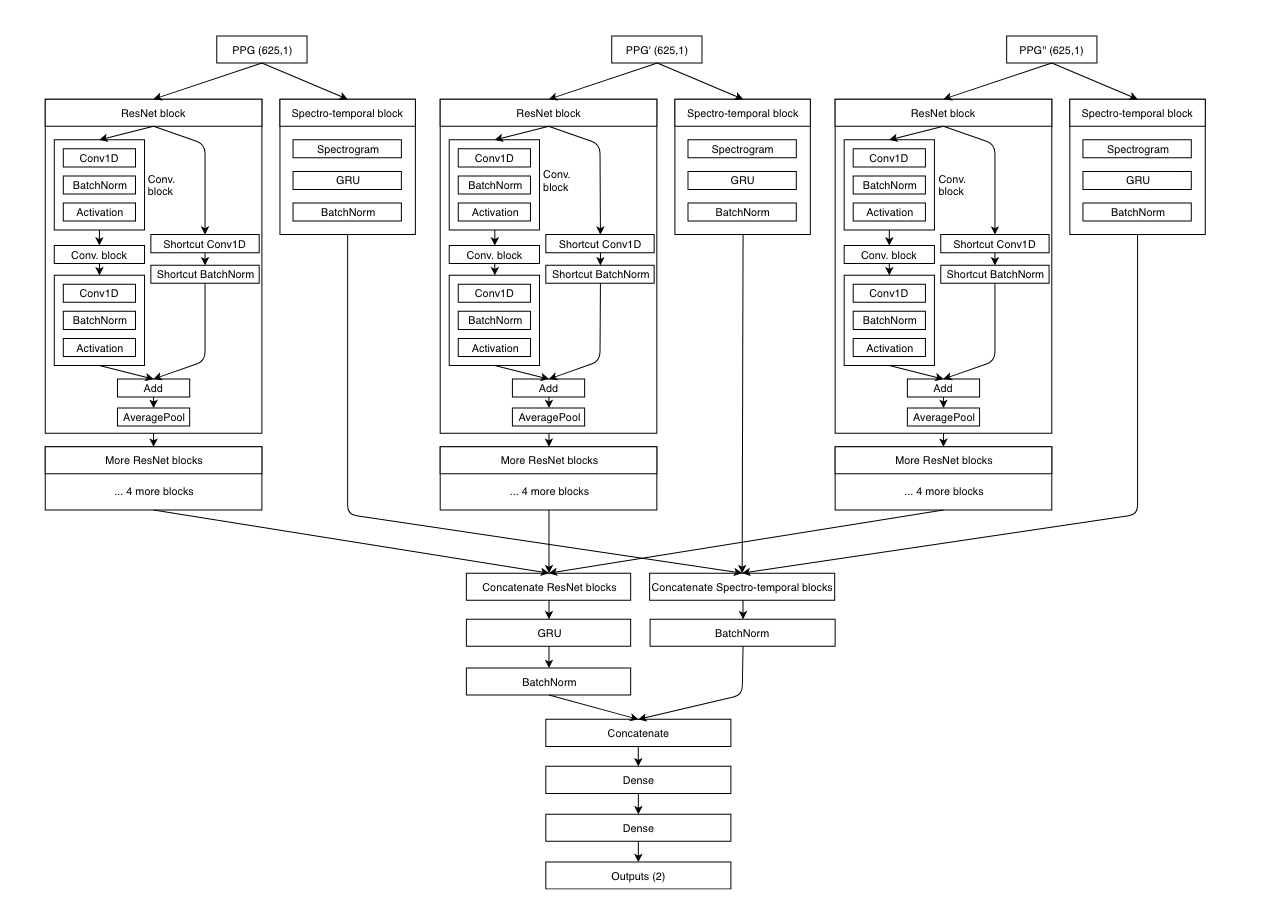
\includegraphics[width=0.8\textheight]{reproductions/slapnicar.png}
    \end{figure}
    PPG Only
\end{frame}

\begin{frame}{Contribution 2: Model Reproduction}{Athaya et al.}
    \begin{figure}
        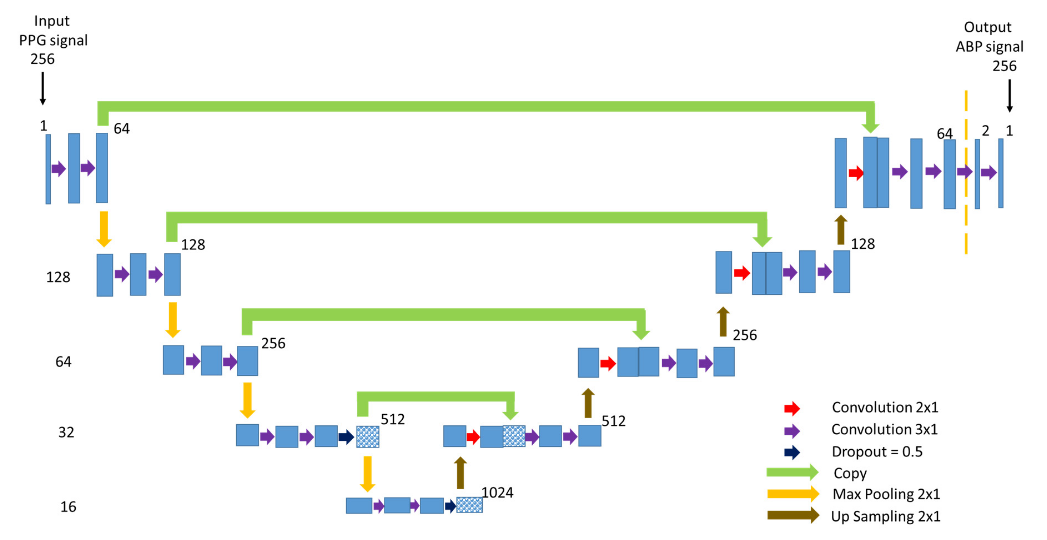
\includegraphics[width=\columnwidth]{reproductions/athaya.png}
    \end{figure}
\end{frame}

\begin{frame}{Contribution 2: Model Reproduction}{Chen et al.}
    \begin{figure}
        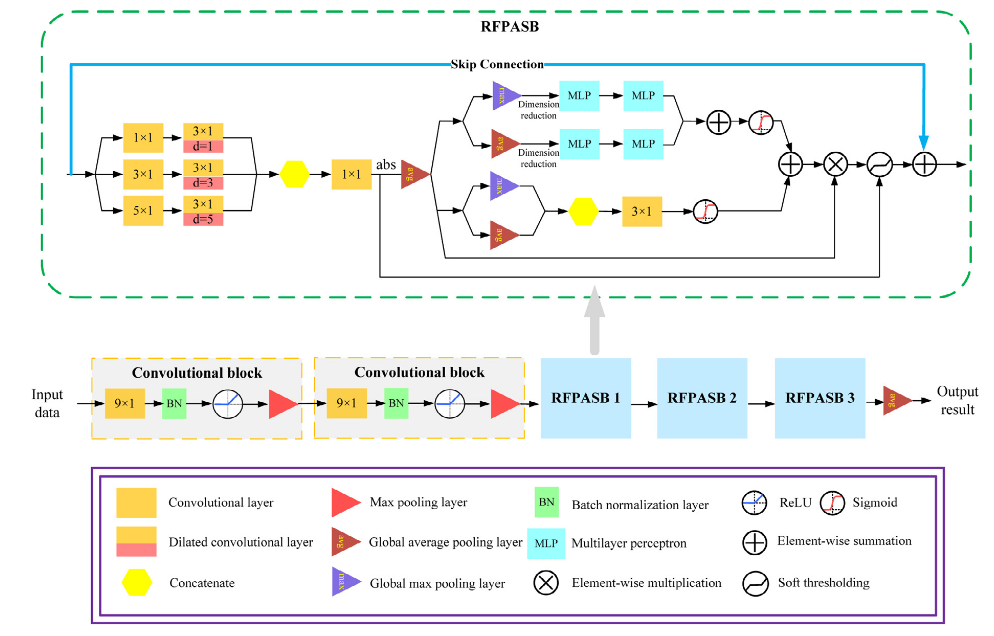
\includegraphics[width=0.8\columnwidth]{reproductions/chen.png}
    \end{figure}
\end{frame}

\begin{frame}{Contribution 2: Model Reproduction}{Harfiya et al.}
    \begin{figure}
        \includesvg[height=0.8\textheight]{reproductions/harfiya.svg}
    \end{figure}
\end{frame}

\begin{frame}{Contribution 2: Model Reproduction}{Kim et al.}
    \begin{figure}
        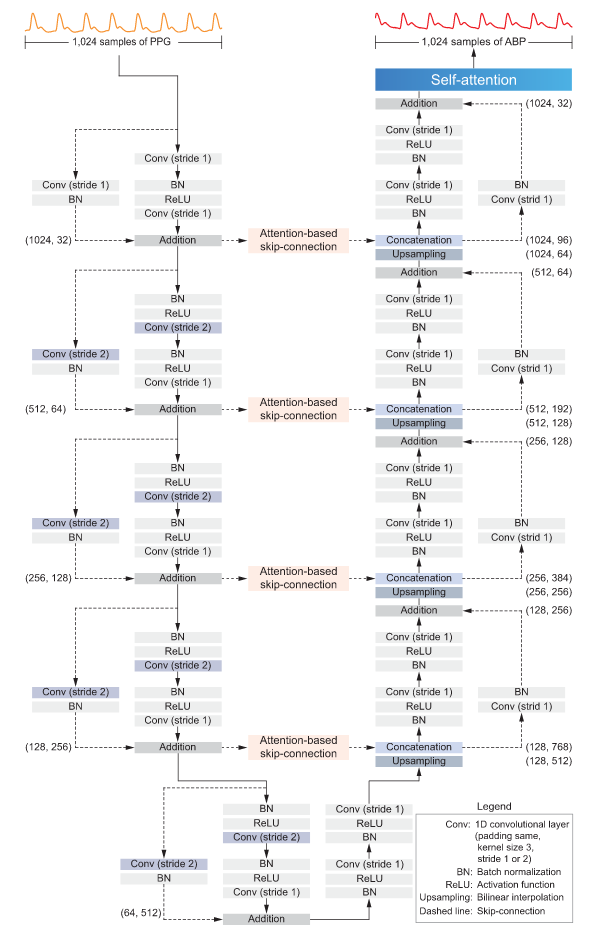
\includegraphics[height=0.8\textheight]{reproductions/kim.png}
    \end{figure}
\end{frame}

\begin{frame}{Contribution 2: Model Reproduction}{Leitner et al.}
    \begin{figure}
        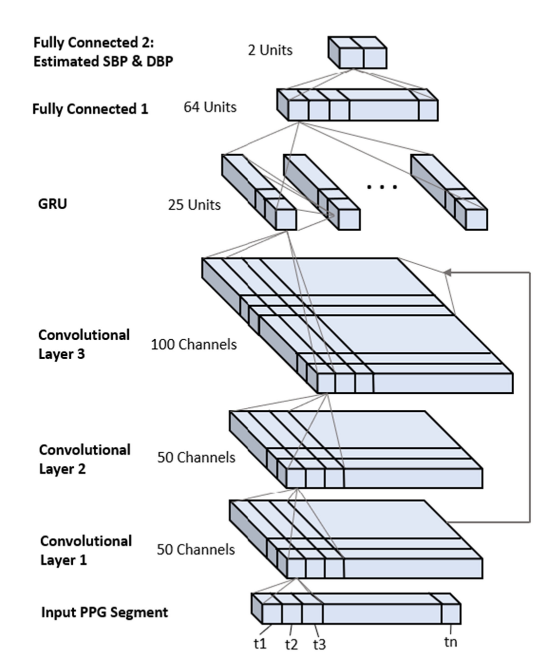
\includegraphics[height=0.8\textheight]{reproductions/leitner.png}
    \end{figure}
\end{frame}

\begin{frame}{Contribution 2: Model Reproduction}{Tazarv and Levorato}
    \begin{figure}
        \includesvg[height=0.8\textheight]{reproductions/tazarv.svg}
    \end{figure}
\end{frame}

\begin{frame}{Contribution 2: Model Reproduction}{Schrumpf et al.}
    \begin{figure}
        \centering
        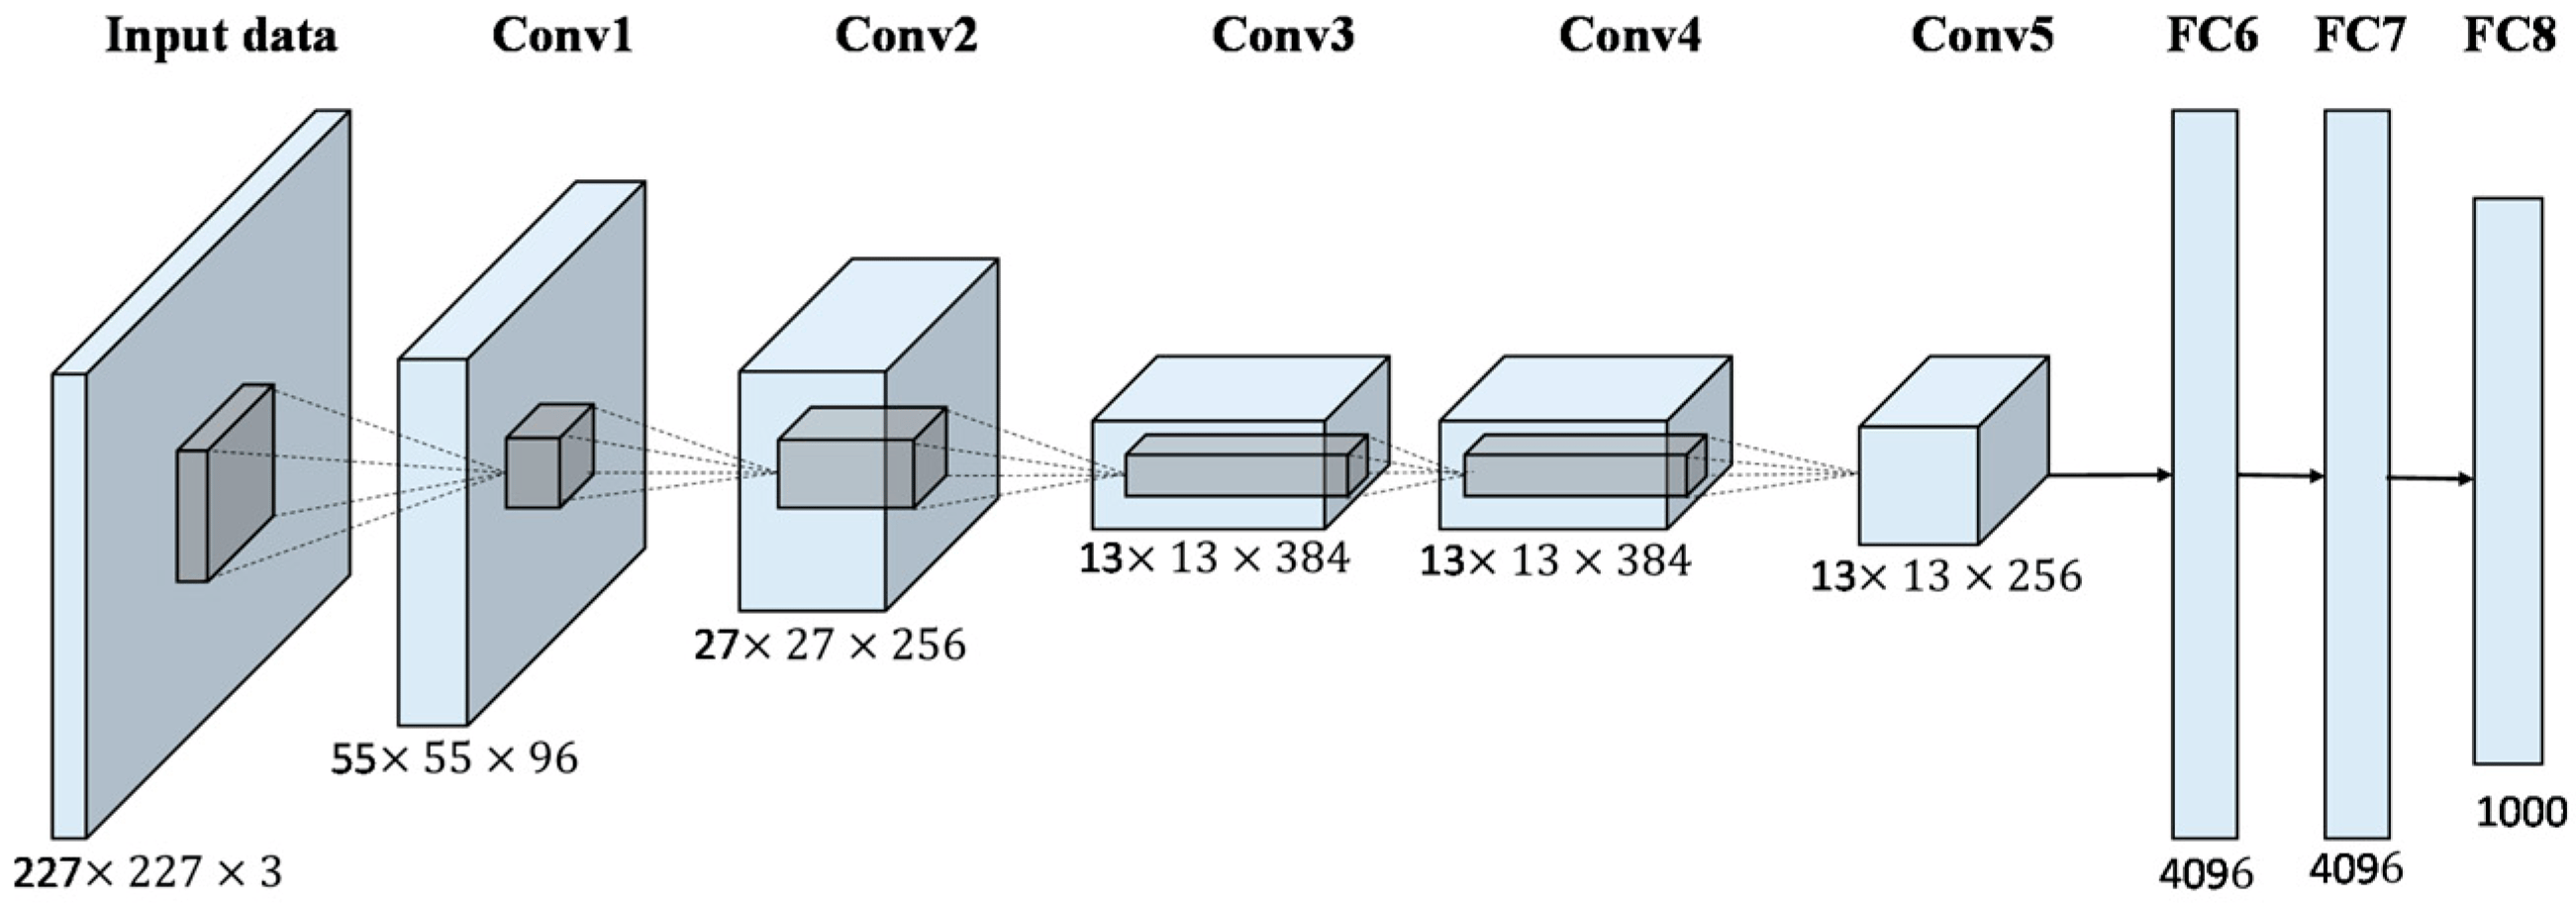
\includegraphics[width=0.3\columnwidth]{reproductions/alex.png}
        % \hfill
        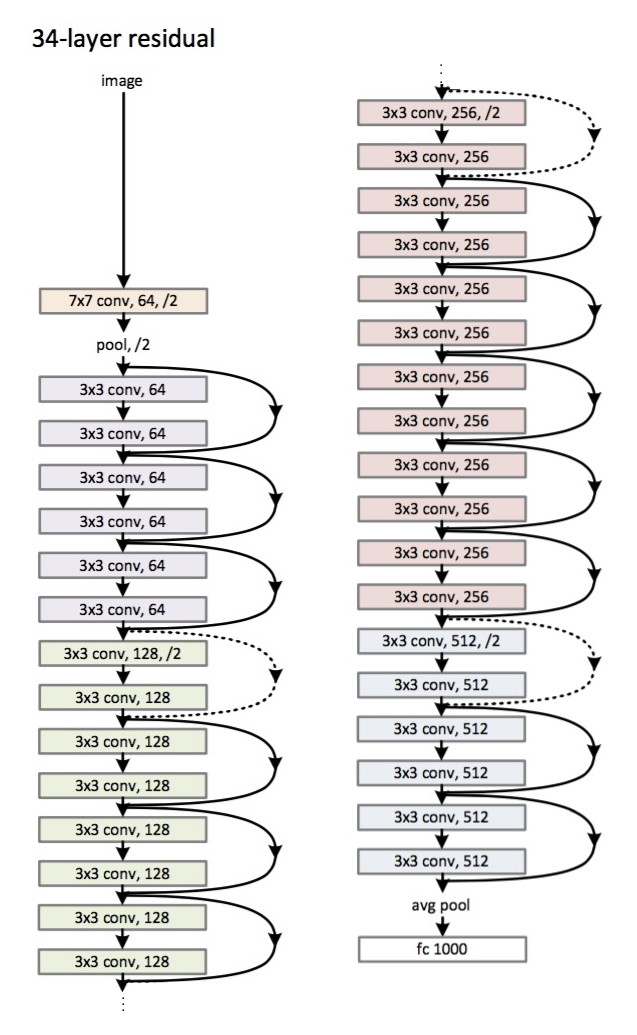
\includegraphics[width=0.3\columnwidth]{reproductions/resnet.png}
    \end{figure}
    ResNet34
\end{frame}

\begin{frame}{Contribution 2: Model Reproduction}{Methodology}
    Changes to the architectures
    \begin{itemize}
        \item Missing information $\to$ best guesses
        \item Adapt for regression task
    \end{itemize}
\end{frame}


\subsection{Proposed Models}
\begin{frame}{Contribution 3: Proposed Models}
    \begin{block}{Objective}
        Propose new preprocessing methodologies and deep learning architectures for BP monitoring.
        Evaluate our models against reproduced models for a concrete clinical context.
    \end{block}
\end{frame}

\begin{frame}{Contribution 3: Proposed Models}{Methodology}
    Compare popular feature-extraction layers
    \begin{itemize}
        \item MLP
        \item RNN-MLP
        \item Residual CNN
        \item Transformer Encoder
    \end{itemize}

    \begin{itemize}
        \item Hyperparameter optimization
        \item Test different types of feature extraction layers
    \end{itemize}
\end{frame}

\begin{frame}{Contribution 3: Proposed Models}{MLP}
    \begin{columns}
        \column{0.5\columnwidth}
        \begin{figure}
            \includesvg[width=0.8\columnwidth]{models/MLP.svg}
        \end{figure}

        \column{0.5\columnwidth}
        \begin{itemize}
            \item 128 units hidden
            \item 2 units output
        \end{itemize}
        \begin{itemize}
            \item simplest model
        \end{itemize}
    \end{columns}

\end{frame}

\begin{frame}{Contribution 3: Proposed Models}{RNN-MLP}
    \begin{columns}
        \column{0.5\columnwidth}
        \begin{figure}
            \includesvg[width=0.8\columnwidth]{models/RNN-MLP.svg}
        \end{figure}

        \column{0.5\columnwidth}
        \begin{itemize}
            \item 256 units GRU layers
            \item stacked MLP
        \end{itemize}
    \end{columns}
\end{frame}

\begin{frame}{Contribution 3: Proposed Models}{Residual CNN}
    \begin{columns}
        \column{0.5\columnwidth}
        \begin{figure}
            \includesvg[width=0.27\columnwidth]{models/Residual Conv.svg}
            \includesvg[width=0.27\columnwidth]{models/Residual Conv - Residual Block.svg}
        \end{figure}

        \column{0.5\columnwidth}
        \begin{itemize}
            \item kernel: 3
            \item Stacked MLP with Dropout 0.01
        \end{itemize}
        \begin{tabular}{lSS}
            \hline
            Module & {Blocks} & {Filters} \\
            \hline
            1st    & 2        & 64        \\
            2nd    & 4        & 128       \\
            3rd    & 8        & 256       \\
            4th    & 2        & 256       \\
            \hline
        \end{tabular}
    \end{columns}

\end{frame}

\begin{frame}{Contribution 3: Proposed Models}{Transformer Encoder}
    \begin{columns}
        \column{0.5\columnwidth}
        \begin{figure}
            \includesvg[width=0.3\columnwidth]{models/Transformer Encoder.svg}
        \end{figure}

        \column{0.5\columnwidth}
        \begin{itemize}
            \item Encoder part only
            \item 4 attention heads
            \item First dense layer: 64 units
            \item Second dense layer: embedding size
        \end{itemize}
    \end{columns}


\end{frame}\begin{frame}{Contribution 3: Input Methodologies}{Methodology}
    Compare Input Methodologies
    \begin{itemize}
        \item Window
        \item Heartbeat
        \item Heartbeat sequence
    \end{itemize}
\end{frame}

\begin{frame}{Contribution 3: Heartbeat Sequence Input}{Methodology}
    Keep fined-grained analysis and temporal aspect
    \begin{figure}
        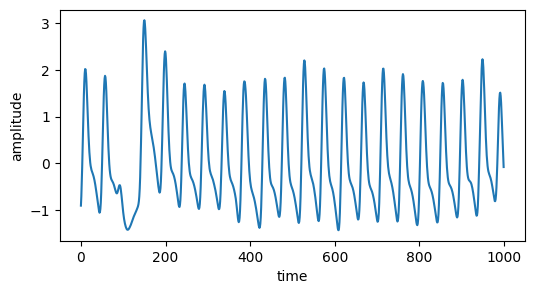
\includegraphics[width=0.35\columnwidth]{inputs/window.png}

        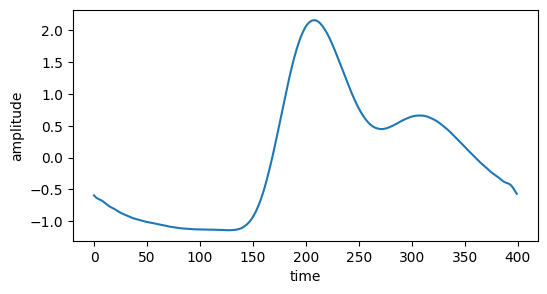
\includegraphics[width=0.35\columnwidth]{inputs/heartbeat.png}
        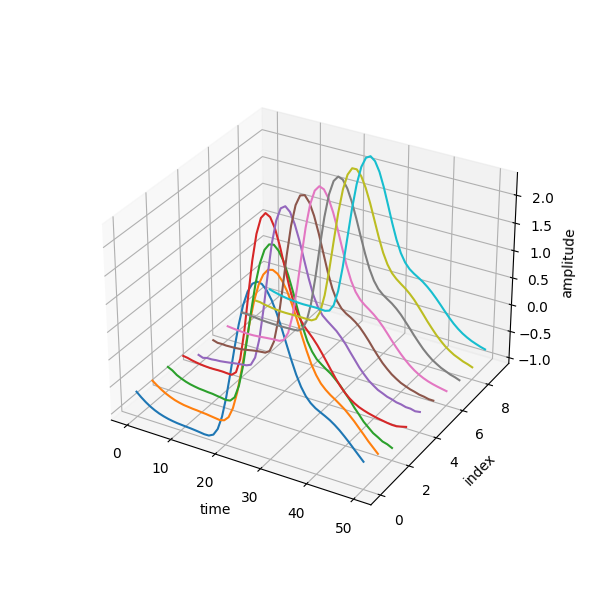
\includegraphics[width=0.35\columnwidth]{inputs/heartbeat-sequence.png}
    \end{figure}
\end{frame}


\begin{frame}{Contribution 2 \& 3}{Results}
    \centering
    Window
    \begin{figure}
        \includesvg[width=0.49\columnwidth]{results/window SBP.svg}
        \hfill
        \includesvg[width=0.49\columnwidth]{results/window DBP.svg}
    \end{figure}
    \begin{itemize}
        \item large gap between random and patient-wise split
        \item 13.802 mmHg lower for random split on average
    \end{itemize}
\end{frame}

\begin{frame}{Contribution 2 \& 3}{Results}
    \centering
    Heartbeat
    \begin{figure}
        \includesvg[width=0.49\columnwidth]{results/heartbeat SBP.svg}
        \hfill
        \includesvg[width=0.49\columnwidth]{results/heartbeat DBP.svg}
    \end{figure}
    \begin{itemize}
        \item Random split is most often used in the literature
    \end{itemize}
\end{frame}


\begin{frame}{Contribution 2 \& 3}{Results}
    \centering
    Heartbeat Sequence
    \begin{figure}
        \includesvg[width=0.49\columnwidth]{results/beatsequence SBP.svg}
        \hfill
        \includesvg[width=0.49\columnwidth]{results/beatsequence DBP.svg}
    \end{figure}
    \begin{itemize}
        \item Random split passes AAMI, but does not generalize
        \item No models meet AAMI standard for patient-wise
    \end{itemize}
\end{frame}

\begin{frame}{Contribution 2 \& 3}{Results}
    \centering
    Heartbeat Sequence
    \begin{figure}
        \includesvg[width=0.49\columnwidth]{results/beatsequence SBP.svg}
        \hfill
        \includesvg[width=0.49\columnwidth]{results/beatsequence DBP.svg}
    \end{figure}
    \begin{itemize}
        \item Random split passes AAMI, but does not generalize
        \item No models meet AAMI standard for patient-wise
    \end{itemize}
\end{frame}

\begin{frame}{Contribution 2 \& 3}{Results}
    \begin{block}{Main Finding \#1}
        Non-invasive, calibration-free BP monitoring remains an unsolved problem.
    \end{block}
\end{frame}

\begin{frame}{Contribution 2 \& 3}{Results}
    \begin{columns}
        \column{0.5\columnwidth}
        \centering
        Best patient-wise
        \begin{figure}
            \includesvg[height=0.3\textheight]{models/MLP.svg}
        \end{figure}

        \begin{table}[htbp]
            \centering
            \resizebox{\linewidth}{!}{
                \begin{tabular}{SSSS}
                    \hline
                    \multicolumn{2}{c}{SBP (mmHg)} & \multicolumn{2}{c}{DBP (mmHg)}                  \\
                    \cmidrule(lr){1-2} \cmidrule(lr){3-4}
                    {MAE}                          & {SD}                           & {MAE}  & {SD}  \\
                    \hline
                    18.547                         & 14.054                         & 10.152 & 6.986 \\
                    \hline
                \end{tabular}
            }
        \end{table}

        \column{0.5\columnwidth}
        \centering
        Best overall
        \begin{figure}
            \includesvg[height=0.3\textheight]{models/RNN-MLP.svg}
        \end{figure}
        \begin{table}[htbp]
            \centering
            \resizebox{\linewidth}{!}{
                \begin{tabular}{SSSS}
                    \hline
                    \multicolumn{2}{c}{SBP (mmHg)} & \multicolumn{2}{c}{DBP (mmHg)}                 \\
                    \cmidrule(lr){1-2} \cmidrule(lr){3-4}
                    {MAE}                          & {SD}                           & {MAE} & {SD}  \\
                    \hline
                    3.423                          & 4.344                          & 1.937 & 3.278 \\
                    \hline
                \end{tabular}
            }
        \end{table}
    \end{columns}
\end{frame}


\begin{frame}{Contribution 2 \& 3}{Results}
    \begin{figure}[htbp]
        \centering
        \includesvg[width=0.35\columnwidth]{results/preprocessing random split SBP Mean Absolute Error.svg}
        \includesvg[width=0.35\columnwidth]{results/preprocessing random split DBP Mean Absolute Error.svg}

        \includesvg[width=0.35\columnwidth]{results/preprocessing patient split SBP Mean Absolute Error.svg}
        \includesvg[width=0.35\columnwidth]{results/preprocessing patient split DBP Mean Absolute Error.svg}
    \end{figure}
    \begin{itemize}
        \item Best input: Usually Heartbeat Sequence
    \end{itemize}
\end{frame}

\begin{frame}{Contribution 2 \& 3}{Results}
    \begin{table}[htbp]
        \centering
        \resizebox{\linewidth}{!}{
            \begin{tabular}{l SSS SSS}
                \hline
                        & \multicolumn{3}{c}{SBP MAE (mmHg) } & \multicolumn{3}{c}{DBP MAE (mmHg)}                                           \\
                \cmidrule(lr){2-4} \cmidrule(lr){5-7}
                Split   & {Training}                          & {Test}                             & {Diff.} & {Training} & {Test} & {Diff.} \\
                \hline
                Random  & 10.421                              & 10.601                             & 0.180   & 5.514      & 5.67   & 0.156   \\
                Patient & 10.008                              & 24.617                             & 14.609  & 5.506      & 13.522 & 8.016   \\
                \hline
            \end{tabular}
        }
    \end{table}
    \begin{itemize}
        \item Train-test gap much larger for patient-wise
        \item Sign of overfitting
    \end{itemize}
\end{frame}

\begin{frame}{Contribution 2 \& 3}{Results}
    \begin{columns}[c]
        \column{0.45\columnwidth}
        \begin{figure}
            \includesvg[height=0.4\textheight]{models/MLP.svg}
        \end{figure}

        \column{0.1\columnwidth}
        vs.

        \column{0.45\columnwidth}
        \begin{figure}
            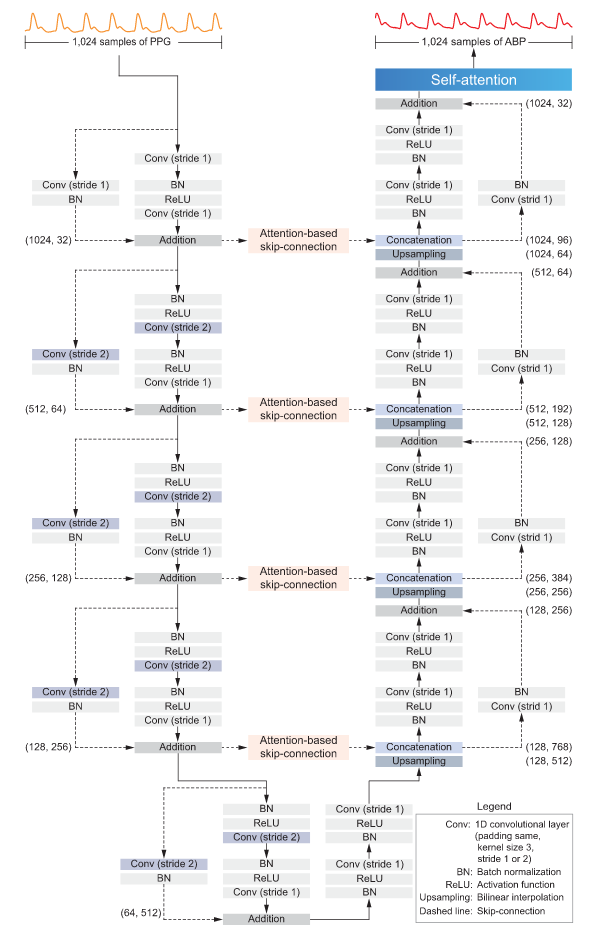
\includegraphics[height=0.4\textheight]{reproductions/kim.png}
        \end{figure}
    \end{columns}

    \begin{table}[htbp]
        \centering
        \resizebox{\linewidth}{!}{
            \begin{tabular}{l SSS SSS}
                \hline
                              & \multicolumn{3}{c}{SBP MAE (mmHg) } & \multicolumn{3}{c}{DBP MAE (mmHg)}                                                                       \\
                \cmidrule(lr){2-4} \cmidrule(lr){5-7}
                Preprocessing & {MLP}                               & {Kim et al. \cite{kim_deepcnap_2022}} & {Imp.} & {MLP}  & {Kim et al. \cite{kim_deepcnap_2022}} & {Imp.} \\
                \hline
                Window        & 22.83                               & 19.1                                  & 3.73   & 12.525 & 12.313                                & 0.212  \\
                Heartbeat     & 18.792                              & 20.701                                & 1.909  & 13.13  & 13.021                                & 0.109  \\
                \hline
            \end{tabular}
        }
    \end{table}

    \begin{itemize}
        \item 145k parameters vs. 5.5B
        \item Complexity doesn't justify the performance Improvement
    \end{itemize}
\end{frame}

\begin{frame}{Contribution 2 \& 3}{Results}
    Overfitting solutions:
    \begin{itemize}
        \item \sout{Increase complexity}
        \item \sout{Increase regularization}
        \item Increase data
    \end{itemize}
\end{frame}


% Reproduction allows for better comparison
% Large gap between random and patient-wise
% 13.802mmHg lower for random
% Random is generally used in the literature
% Random split passes AAMI doest not generalize
% No models meet AAMI standard for patient-wise

% best patient-wise ais MLP w/ heartbeat sequence
% best overall is RNN-NLP w/ heartbeat sequence
% heartbeat sequence performs the best

% train-test gap random vs patient-wise
% Complexity of model doesn't justify performance Improvement
% OVerfitting, increase complexity(No), increase regularization (no), Increase Data(?)

% Poor dataset variability


\subsection{Learning Curve Analysis}
\begin{frame}{Contribution 4: Learning Curve Analysis}
    \begin{block}{Objective}
        Evaluate how much data is required to achieve a calibration-free BP estimation algorithms.
    \end{block}
\end{frame}

\begin{frame}{Contribution 4: Learning Curve Analysis}{Methodology}
    \begin{figure}
        \includesvg[width=0.8\columnwidth]{lcanalysis/lc analysis split.svg}
    \end{figure}
    \begin{itemize}
        \item MLP Model
        \item Heartbeat Input
    \end{itemize}
\end{frame}

\begin{frame}{Contribution 4: Learning Curve Analysis}{Results}
    \begin{figure}[htbp]
        \includesvg[width=0.4\columnwidth]{lcanalysis/lc analysis SBP MAE.svg}
        \includesvg[width=0.4\columnwidth]{lcanalysis/lc analysis SBP SD.svg}

        \includesvg[width=0.4\columnwidth]{lcanalysis/lc analysis DBP MAE.svg}
        \includesvg[width=0.4\columnwidth]{lcanalysis/lc analysis DBP SD.svg}
    \end{figure}
    Improvement for SBP MAE only
\end{frame}


\begin{frame}{Contribution 4: Learning Curve Analysis}{Results}

    \begin{equation}\label{eq:fitted curve}
        y=\num{28.533} - \num{9.518} x^{\num{0.295}}
    \end{equation}
    \begin{figure}[htbp]
        \includesvg[width=0.6\columnwidth]{lcanalysis/fitted model.svg}
    \end{figure}

    \pause
    \begin{itemize}
        \item $42 \times 21.52 \approx 904$ patients
        \item Low diversity dataset
    \end{itemize}
\end{frame}

\begin{frame}{Contribution 4}{Results}
    \begin{block}{Main Finding \#2}
        Improvements in data are more effective at improving performance for non-invasive blood pressure monitoring.
    \end{block}
\end{frame}







\section{Future Work}
\begin{frame}{Future Work}
    \begin{itemize}
        \item Multiple Sensors
              \begin{itemize}
                  \item PPG, PPG $\to$ PTT
                  \item PPG, ECG $\to$ PAT
              \end{itemize}
        \item Demographic information
        \item Acquire more data
              \begin{itemize}
                  \item Improve performance
                  \item Validate extrapolation
                  \item Use different datasets
              \end{itemize}
    \end{itemize}
\end{frame}

\begin{frame}[allowframebreaks]{References}
    \tiny
    \bibliography{references/PPG-BP-litterature-review,
        references/PPG-BP,
        references/libraries,
        references/extra,
        references/BP-Estimation-Intro,
        references/datasets
    }
    \bibliographystyle{plain}
\end{frame}



\begin{frame}{Results Table}
    \begin{columns}
        \column{0.5\columnwidth}
        \centering \tiny Window
        \begin{table}
            \centering
            \sisetup{detect-weight}
            \robustify\bfseries
            \resizebox{\columnwidth}{!}{
                \begin{tabular}{lSSSS}
                    \hline
                                                                    & \multicolumn{2}{c}{SBP (mmHg)}         & \multicolumn{2}{c}{DBP (mmHg)}                                       \\
                    \cmidrule(lr){2-3} \cmidrule(lr){4-5}
                    Model                                           & {MAE}                                  & {SD}                           & {MAE}            & {SD}             \\
                    \hline
                                                                    & \multicolumn{4}{c}{Patient-wise split}                                                                        \\
                    \cmidrule{2-5}
                    Slapničar et al. \cite{slapnicar_blood_2019}    & 21.013                                 & 14.158                         & 13.263           & 10.742           \\
                    Athaya and Choi \cite{athaya_estimation_2021}   & 23.169                                 & 17.47                          & 12.056           & 10.384           \\
                    Chen et al. \cite{chen_new_2022}                & 21.986                                 & 15.011                         & \bfseries 11.662 & \bfseries 10.292 \\
                    Harfiya et al. \cite{harfiya_continuous_2021}   & 29.447                                 & 18.027                         & 11.843           & 9.597            \\
                    Kim et al. \cite{kim_deepcnap_2022}             & \bfseries 19.1                         & \bfseries 13.889               & 12.313           & 10.186           \\
                    Leitner et al. \cite{leitner_personalized_2022} & 103.847                                & 20.44                          & 28.935           & 14.732           \\
                    Tazarv and Levorato \cite{tazarv_deep_2021}     & 21.301                                 & 16.772                         & 11.815           & 9.677            \\
                    AlexNet \cite{schrumpf_assessment_2021}         & 21.222                                 & 15.017                         & 12.11            & 10.452           \\
                    Resnet34 \cite{schrumpf_assessment_2021}        & 21.078                                 & 15.297                         & 11.968           & 10.47            \\
                    \textbf{MLP}                                    & 22.83                                  & 17.164                         & 12.525           & 10.879           \\
                    % \textbf{Softmax MLP} & 89.942 & 19.948 & 17.54 & 12.974 \\
                    \textbf{RNN-MLP}                                & 25.447                                 & 17.252                         & 11.827           & 9.573            \\
                    \textbf{Residual CNN}                           & 22.205                                 & 15.56                          & 12.88            & 10.367           \\
                    \textbf{Transformer Encoder}                    & 25.59                                  & 17.164                         & 12.525           & 10.879           \\

                                                                    & \multicolumn{4}{c}{Random split}                                                                              \\
                    \cmidrule{2-5}
                    Slapničar et al. \cite{slapnicar_blood_2019}    & 6.26                                   & 7.621                          & 3.601            & 5.711            \\
                    Athaya and Choi \cite{athaya_estimation_2021}   & 13.146                                 & 12.162                         & 8.379            & 7.58             \\
                    Chen et al. \cite{chen_new_2022}                & 5.051                                  & 7.232                          & 3.117            & 5.646            \\
                    Harfiya et al. \cite{harfiya_continuous_2021}   & 14.908                                 & 12.387                         & 8.669            & 7.66             \\
                    Kim et al. \cite{kim_deepcnap_2022}             & 4.725                                  & 6.746                          & 3.005            & 5.57             \\
                    Leitner et al. \cite{leitner_personalized_2022} & 91.673                                 & 21.105                         & 31.872           & 13.742           \\
                    Tazarv and Levorato \cite{tazarv_deep_2021}     & 6.255                                  & 8.155                          & 3.964            & 6.21             \\
                    AlexNet \cite{schrumpf_assessment_2021}         & 5.303                                  & 7.043                          & 3.164            & 5.646            \\
                    Resnet34 \cite{schrumpf_assessment_2021}        & 5.077                                  & 7.194                          & 3.172            & 5.696            \\
                    \textbf{MLP}                                    & 11.52                                  & 11.125                         & 7.269            & 7.604            \\
                    \textbf{RNN-MLP}                                & 7.685                                  & 8.512                          & 4.668            & 6.313            \\
                    \textbf{Residual CNN}                           & \bfseries 4.56                         & \bfseries 6.452                & \bfseries 2.752  & \bfseries 5.377  \\
                    \textbf{Transformer Encoder}                    & 14.908                                 & 12.413                         & 8.672            & 7.665            \\
                    \hline
                \end{tabular}
            }
        \end{table}

        \column{0.5\columnwidth}
        \centering \tiny Heartbeat Sequence
        \begin{table}
            \centering
            \sisetup{detect-weight}
            \robustify\bfseries
            \resizebox{\columnwidth}{!}{
                \begin{tabular}{lSSSS}
                    \hline
                                                                    & \multicolumn{2}{c}{SBP (mmHg)}         & \multicolumn{2}{c}{DBP (mmHg)}                                       \\
                    \cmidrule(lr){2-3} \cmidrule(lr){4-5}
                    Model                                           & {MAE}                                  & {SD}                           & {MAE}            & {SD}             \\
                    \hline
                                                                    & \multicolumn{4}{c}{Patient-wise split}                                                                        \\
                    \cmidrule{2-5}
                    Slapničar et al. \cite{slapnicar_blood_2019}    & 22.092                                 & 15.087                         & 14.611           & 10.463           \\
                    Athaya and Choi \cite{athaya_estimation_2021}   & 24.715                                 & 16.206                         & \bfseries 11.904 & \bfseries 10.043 \\
                    Chen et al. \cite{chen_new_2022}                & 20.155                                 & 14.138                         & 14.201           & 9.927            \\
                    Harfiya et al. \cite{harfiya_continuous_2021}   & 19.691                                 & 14.351                         & 14.065           & 10.42            \\
                    Kim et al. \cite{kim_deepcnap_2022}             & \bfseries 18.792                       & \bfseries 14.353               & 13.021           & 9.982            \\
                    Leitner et al. \cite{leitner_personalized_2022} & 21.863                                 & 16.69                          & 15.09            & 10.422           \\
                    Tazarv and Levorato \cite{tazarv_deep_2021}     & 20.425                                 & 15.859                         & 12.501           & 9.735            \\
                    AlexNet \cite{schrumpf_assessment_2021}         & 19.638                                 & 14.757                         & 13.927           & 10.331           \\
                    Resnet34 \cite{schrumpf_assessment_2021}        & 20.8                                   & 14.176                         & 15.435           & 10.226           \\
                    \textbf{MLP}                                    & 20.701                                 & 15.836                         & 13.13            & 9.836            \\
                    \textbf{RNN-MLP}                                & 24.924                                 & 14.618                         & 13.158           & 10.394           \\
                    \textbf{Residual CNN}                           & 20.738                                 & 14.565                         & 15.289           & 10.632           \\
                    \textbf{Transformer Encoder}                    & 24.948                                 & 14.621                         & 13.106           & 10.333           \\

                                                                    & \multicolumn{4}{c}{Random split}                                                                              \\
                    \cmidrule{2-5}
                    Slapničar et al. \cite{slapnicar_blood_2019}    & 7.201                                  & 8.034                          & 4.686            & 7.1              \\
                    Athaya and Choi \cite{athaya_estimation_2021}   & 11.943                                 & 10.861                         & 8.599            & 8.666            \\
                    Chen et al. \cite{chen_new_2022}                & 6.694                                  & 7.973                          & 4.469            & 7.134            \\
                    Harfiya et al. \cite{harfiya_continuous_2021}   & 6.192                                  & 7.654                          & 4.099            & 6.965            \\
                    Kim et al. \cite{kim_deepcnap_2022}             & 6.094                                  & 7.577                          & 3.986            & 6.685            \\
                    Leitner et al. \cite{leitner_personalized_2022} & 18.812                                 & 25.476                         & 5.609            & 8.218            \\
                    Tazarv and Levorato \cite{tazarv_deep_2021}     & 6.977                                  & 8.313                          & 4.736            & 7.418            \\
                    AlexNet \cite{schrumpf_assessment_2021}         & 5.591                                  & 7.338                          & 3.613            & 6.607            \\
                    Resnet34 \cite{schrumpf_assessment_2021}        & \bfseries 5.385                        & \bfseries 7.391                & \bfseries 3.407  & \bfseries 6.368  \\
                    \textbf{MLP}                                    & 8.485                                  & 8.984                          & 5.911            & 7.624            \\
                    \textbf{RNN-MLP }                               & 5.873                                  & 7.419                          & 3.907            & 6.666            \\
                    \textbf{Residual CNN}                           & 5.783                                  & 7.331                          & 3.704            & 6.446            \\
                    \textbf{Transformer Encoder}                    & 13.716                                 & 11.164                         & 10.126           & 9.007            \\
                    \hline
                \end{tabular}
            }
        \end{table}
    \end{columns}
\end{frame}

\begin{frame}{Results Table}
    \centering \tiny Heartbeat Sequence
    \begin{table}[htbp]
        \centering
        \sisetup{detect-weight}
        \robustify\bfseries
        \resizebox{\columnwidth}{!}{
            \begin{tabular}{lSSSS}
                \hline
                                             & \multicolumn{2}{c}{SBP (mmHg)}         & \multicolumn{2}{c}{DBP (mmHg)}                                      \\
                \cmidrule(lr){2-3} \cmidrule(lr){4-5}
                Model                        & {MAE}                                  & {SD}                           & {MAE}            & {SD}            \\
                \hline
                                             & \multicolumn{4}{c}{Patient-wise split}                                                                       \\
                \cmidrule{2-5}
                \textbf{MLP}                 & \bfseries 18.547                       & \bfseries 14.054               & \bfseries 10.152 & \bfseries 6.986 \\
                \textbf{RNN-MLP}             & 21.491                                 & 16.35                          & 14.952           & 9.648           \\
                \textbf{Residual CNN}        & 21.469                                 & 14.545                         & 14.362           & 8.266           \\
                \textbf{Transformer Encoder} & 19.294                                 & 14.459                         & 11.749           & 8.054           \\

                                             & \multicolumn{4}{c}{Random split}                                                                             \\
                \cmidrule{2-5}
                \textbf{MLP}                 & 6.678                                  & 7.079                          & 4.321            & 5.448           \\
                \textbf{RNN-MLP}             & \bfseries 3.423                        & \bfseries 4.344                & \bfseries 1.937  & \bfseries 3.278 \\
                \textbf{Residual CNN}        & 4.166                                  & 5.382                          & 2.365            & 4.271           \\
                \textbf{Transformer Encoder} & 3.947                                  & 4.644                          & 2.337            & 3.799           \\
                \hline
            \end{tabular}
        }
    \end{table}
\end{frame}

% supplemental slides tables of results

\end{document}